\begin{figure*}[t!]
    \centering
    \begin{subfigure}[b]{0.48\textwidth}
        \centering
        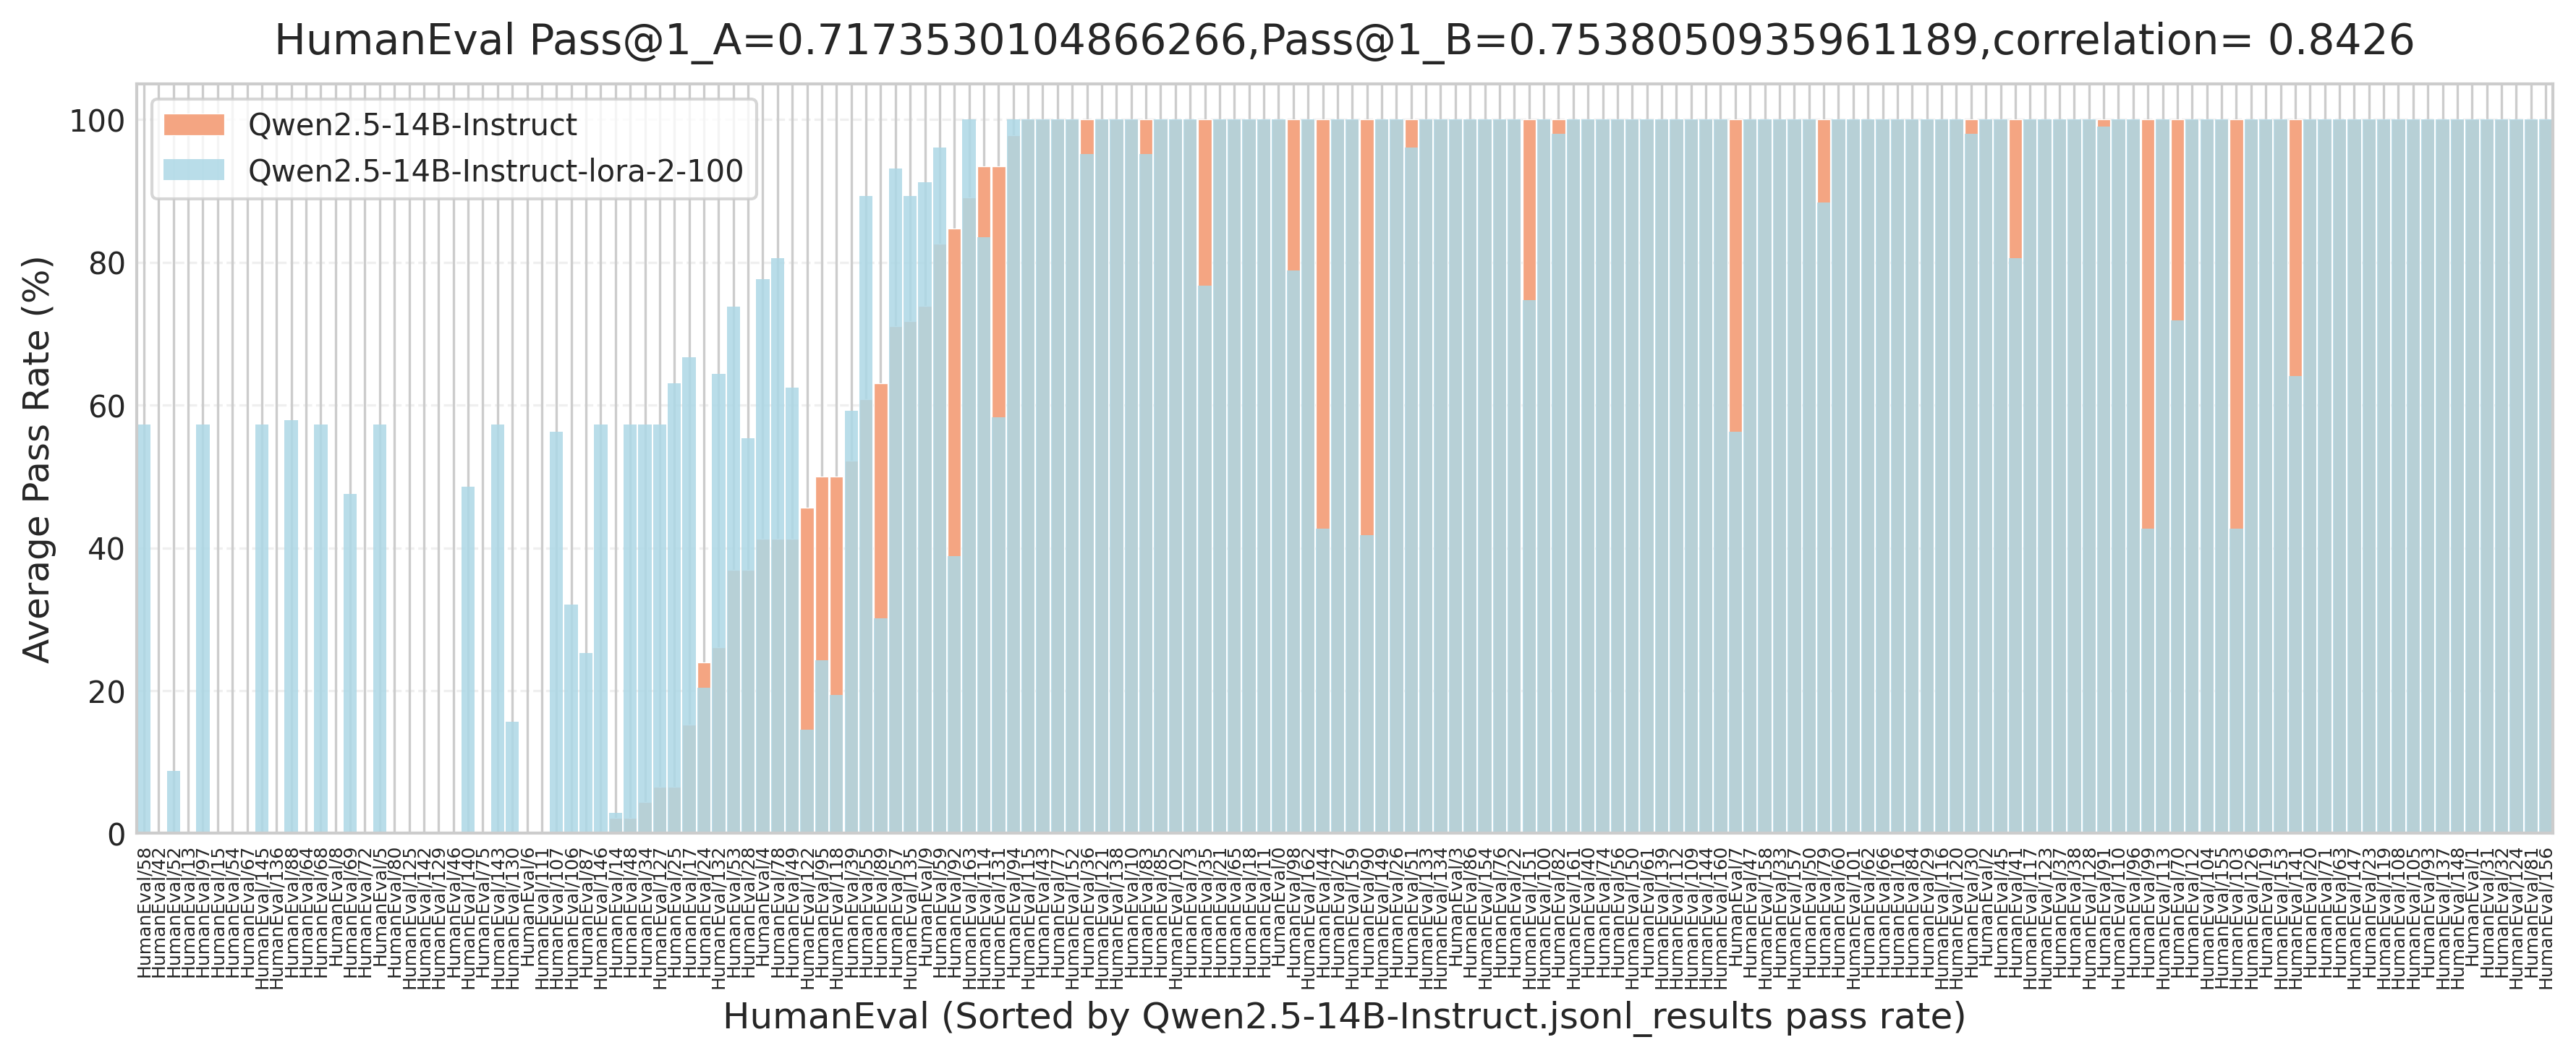
\includegraphics[width=\textwidth]{figures/Qwen.png}
        \caption{Pass@1 for Qwen2.5-14B on original HumanEval}
        \label{fig:qwensub1}
    \end{subfigure}
    \hfill
    \begin{subfigure}[b]{0.48\textwidth}
        \centering
        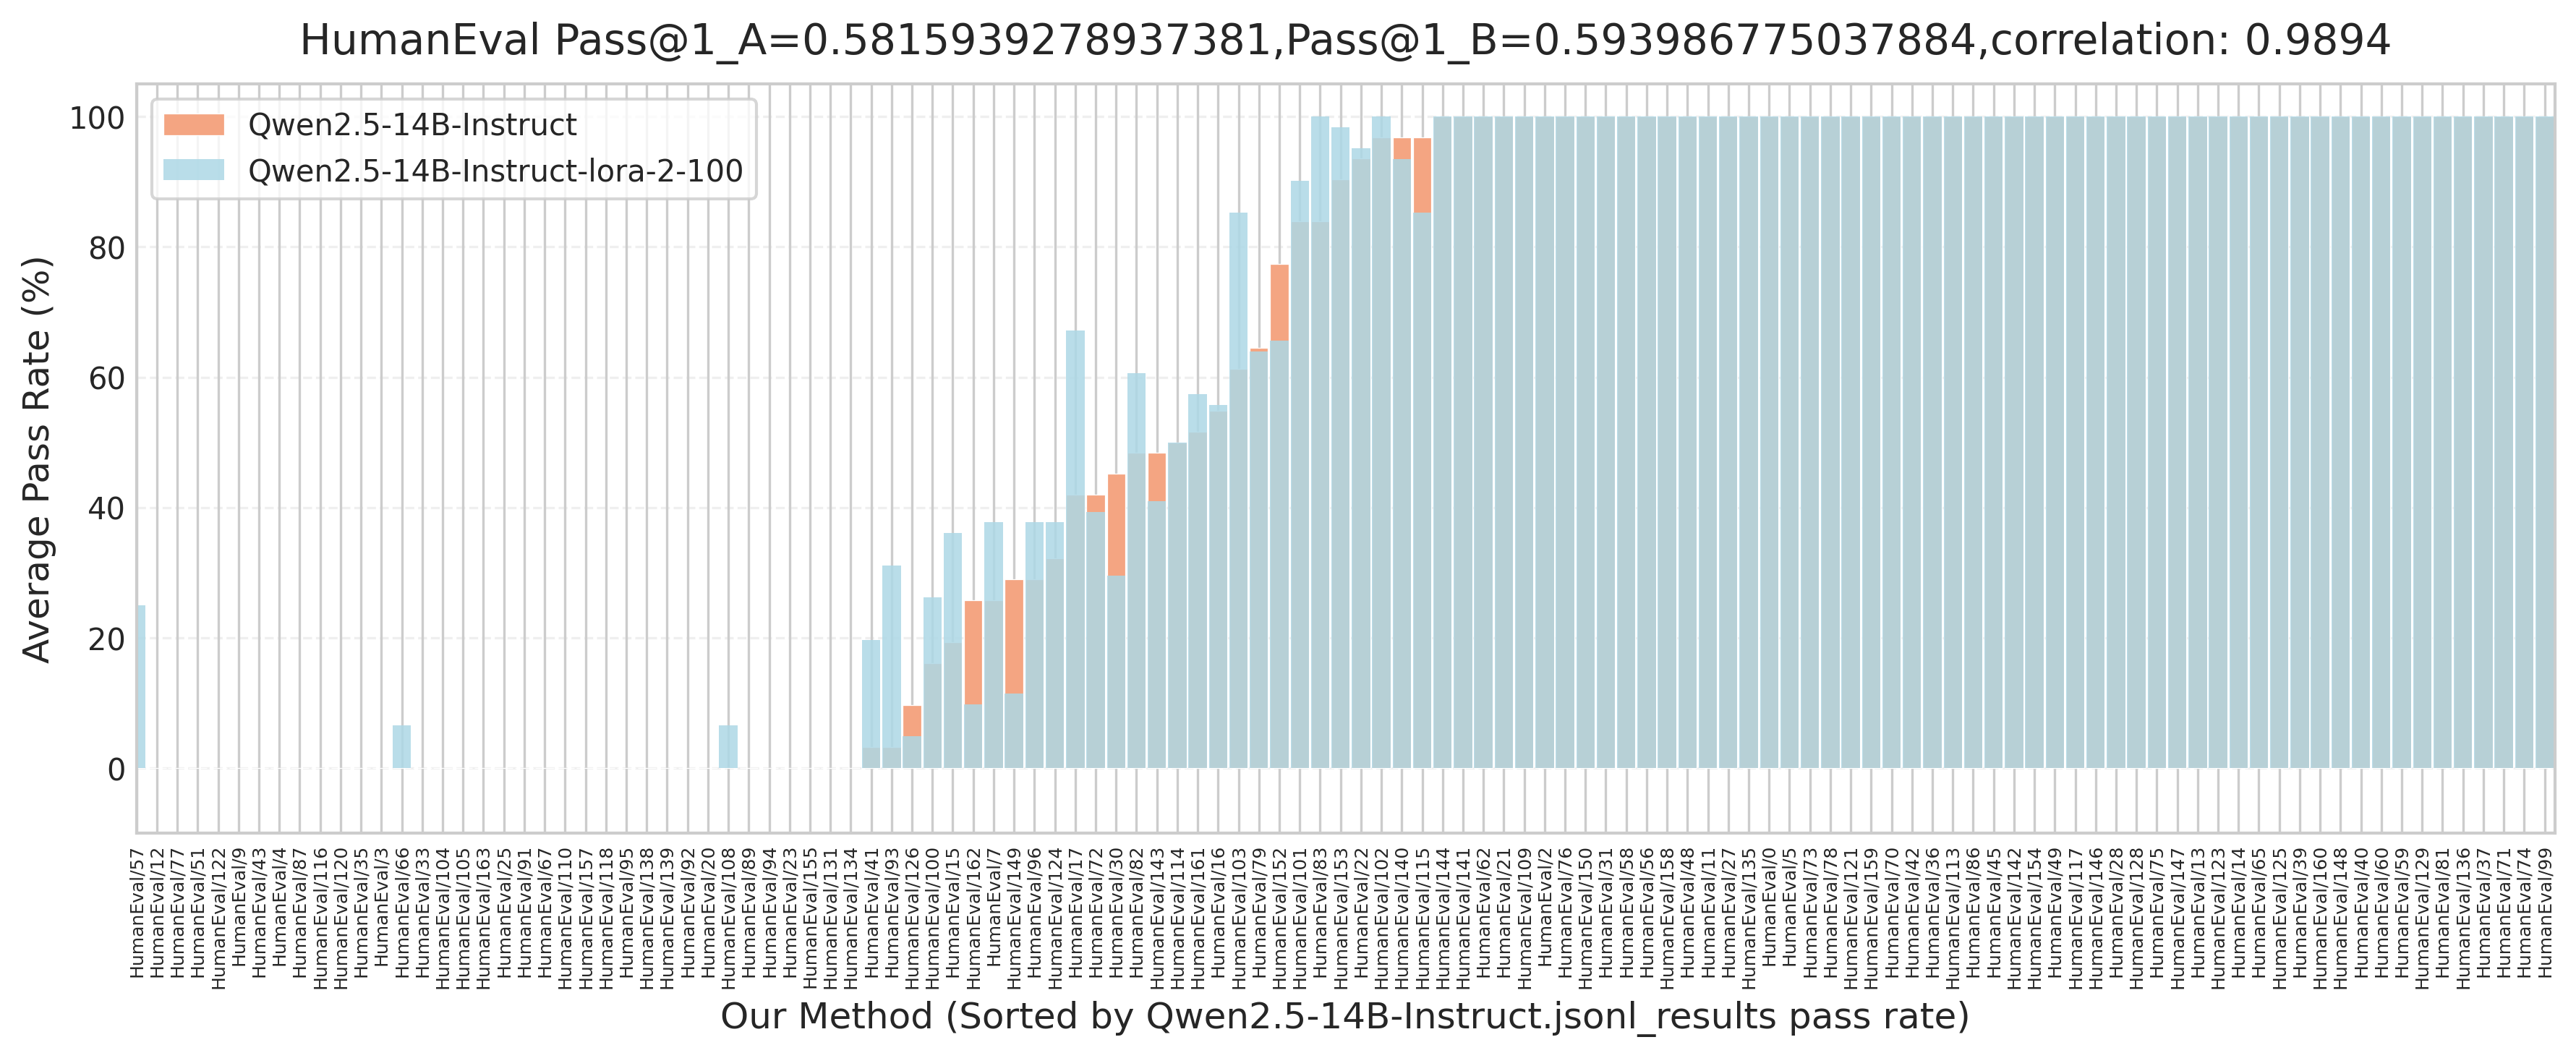
\includegraphics[width=\textwidth]{figures/Qwen2.png}
        \caption{Pass@1 for Qwen2.5-14B on \tool}
        \label{fig:qwensub2}
    \end{subfigure}
    
    \vspace{2mm}
    \caption{The detailed results on the base and \tool{}. The result of \tool{} shows a higher correlation between the clean model and the contaminated model, which means our method can evaluate models more cleanly.}
    \Description{Two scatter plots comparing per-task Pass at 1 scores of Qwen2.5-14B on the original HumanEval benchmark and on CodeArena.}
    \label{fig:Qwen1Comparison}
\end{figure*}